\themaN
\graphicspath{{../Ch16_Proportionnalite/Images/}}

\chapter{La proportionnalité}
\label{C31}


%%%%%%%%%%%%%%%%%%%%%%%%%%%%%%%%%%%%%%%%%%
\begin{prerequis}[Connaissances et compétences abordées]
   \begin{itemize}
     \item Reconnaître et résoudre des problèmes relevant de la proportionnalité en utilisant une procédure adaptée : propriétés de linéarité (additive et multiplicative), passage à l’unité, coefficient de proportionnalité.
     \item Résoudre un problème de proportionnalité impliquant des grandeurs.
     \item Reproduire une figure en respectant une échelle donnée : agrandissement ou réduction d’une figure.
  \end{itemize}
\end{prerequis}

\vfill

\begin{debat}[Débat : proportions et feuilles de papier] 
   Les formats de papier : A0, A1, A2, A3, A4, A5\dots{} ne sont pas dûs au hasard : ils ont été instaurés de manière à ce que les proportions de la feuille soient conservées lorsqu'on la coupe en deux. Le rapport entre la longueur est la largeur est de $\sqrt2$ (racine de 2) soit environ 1,414. \\
   C'est pourquoi une feuille de papier au format A4 a des dimensions de \ucm{21} par \ucm{29,7} car $21\times\sqrt2 \approx29,7$.
   \begin{center}
      \begin{pspicture}(-1,0)(6,4.5)
         \rput(-1.5,2.1){\bf A0}
         \psline{->}(-1.2,2.1)(-0.2,2.1)
         {\psset{fillstyle=solid}
         \psframe[fillcolor=B1](0,0)(5.94,4.2)
         \psframe[fillcolor=B1!80](2.97,0)(5.94,4.2)
         \psframe[fillcolor=B1!60](2.97,2.1)(5.94,4.2)
         \psframe[fillcolor=B2!40](4.45,2.1)(5.94,4.2)
         \psframe[fillcolor=B2!20](4.45,3.15)(5.94,4.2)
         \psframe[fillcolor=B2!00](5.2,3.15)(5.94,4.2)}
         \textcolor{white}{\bf
            \rput(1.4,2.1){A1}
            \rput(4.4,1.05){A2}
            \rput(3.65,3.15){A3}
            \rput(5.1,2.62){A4}
            \rput(4.7,3.67){A5}}
      \end{pspicture}
   \end{center}
   \bigskip
   \begin{cadre}[B2][F4]
      \begin{center}
         Vidéo : \href{https://www.youtube.com/watch?v=VsvplYbMEzc}{\bf Dimensions idéales d'un terrain de foot}, chaîne YouTube {\it Micmaths} de {\it Mickaël Launay}
      \end{center}
   \end{cadre}
\end{debat}

\vfill

\textcolor{PartieGeometrie}{\sffamily\bfseries Cahier de compétences} : chapitre 5, exercices 1 à 23 ; 37 à 40 ; 43.


%%%%%%%%%%%%%%%%%%%%%%%%%%%%%%%%%%%%%
%%%%%%%%%%%%%%%%%%%%%%%%%%%%%%%%%%%%%
\activites

\begin{activite}[Le puzzle de Brousseau]
   {\bf Objectifs :} mettre en \oe uvre un ou des moyens pour résoudre un problème d'agrandissement ; reproduire une figure géométrique en respectant des mesures ; rendre compte d'un travail en groupe.
   \begin{QCM}
      \partie[présentation du puzzle]
         Ci-dessous se trouve un puzzle composé de quatre pièces A, B, C et D dont les mesures dont indiquées sur la figure.
         \begin{center}
            \begin{pspicture}(-1.5,-1.2)(12.5,11.5)
               \psframe(0,0)(11,11)
               \psline(4,0)(4,11)
               \psline(4,6)(11,6)
               \psline(7,0)(7,6)
               {\small
                  \rput(12,3){\ucm{6}}
                  \rput(12,8.5){\ucm{5}}
                  \rput(2,-0.5){\ucm{4}}
                  \rput(5.5,-0.5){\ucm{2}}
                  \rput(9,-0.5){\ucm{5}}}
                  \rput(2,5.5){A}
                  \rput(5.5,3){B}
                  \rput(9,3){C}
                  \rput(7.5,8.5){D}
               \end{pspicture}
            \end{center}
      
      \partie[travail demandé]
         Par groupes de trois ou quatre, vous allez devoir refaire le même puzzle mais en plus grand : il faudra s'accorder sur la procédure à adopter pour agrandir les éléments du puzzle, se répartir la construction des pièces en faisant les calculs individuellement puis assembler les morceaux pour reconstituer le puzzle agrandi. \\
         Le compte-rendu de vos recherches sera présenté sous la forme d’une affiche par groupe. \\
         \begin{center}
            {\bf C'est parti\dots{} le segment de \ucm{4} devra mesurer \ucm{6} sur votre puzzle agrandi.}
         \end{center}
         \bigskip
   \end{QCM}
\end{activite}


%%%%%%%%%%%%%%%%%%%%%%%%%%%%%%%%%%%%%
%%%%%%%%%%%%%%%%%%%%%%%%%%%%%%%%%%%%%
\cours 

\section{Procédures de proportionnalité} %%%%%

\begin{center}
   \begin{pspicture}(0,0.2)(16,10)
      \psellipse[fillstyle=solid,fillcolor=B3](8,5.5)(2.7,1)
      \rput(8,5.5){\parbox{4.1cm}{\centering \bf Si 4 stylos coûtent 10 \ueuro{} \\ combien coûtent 12 stylos ?}}
      \psarc{<-}(5.5,8){2}{205}{270}
      \psellipse[fillstyle=solid,fillcolor=A3](3.5,8.5)(3.4,1.2)
      \rput(3.5,8.5){\parbox{5.7cm}{\centering {\bf Linéarité additive :} \\ 12 stylos = 4 stylos + 4 stylos + 4 stylos \\ coûtent $\ueuro{10}+\ueuro{10}+\ueuro{10} =\ueuro{30}$}}
      \psarc{->}(10.5,8){2}{270}{335}
      \psellipse[fillstyle=solid,fillcolor=A3](12.5,8.5)(3.4,1.2)
      \rput(12.5,8.5){\parbox{5cm}{\centering {\bf Linéarité multiplicative :} \\ 12 stylos = 3$\times$4 stylos \\ coûtent $3\times\ueuro{10} =\ueuro{30}$}}
      \psarc{->}(5.5,3){2}{90}{162}
      \psellipse[fillstyle=solid,fillcolor=A3!50](3.5,2)(3.4,1.5)
      \rput(3.5,2){\parbox{5.1cm}{\centering {\bf Passage par l'unité :} \\ 1 stylo coûte 4 fois moins cher : \\ $\ueuro{10}\div4 =\ueuro{2,5}$ \\ 12 stylos coûtent 12 fois plus cher : \\ $12\times\ueuro{2,5} =\ueuro{30}$}}
      \psarc{<-}(10.5,3){2}{28}{90}
      \psellipse[fillstyle=solid,fillcolor=A3!50](12.5,2)(3.4,1.8)
      \rput(12.5,2){\parbox{6.5cm}{\centering {\bf Coefficient de proportionnalité :} \\ $4\times\fbox{2,5} =10$ \\ le coefficient de proportionnalité vaut 2,5 \\ $12\times\fbox{2,5} =30$ \\ 12 stylos coûtent \ueuro{30}}}
   \end{pspicture}
\end{center}

\section{Reconnaître une situations de proportionnalité} %%%%%%

\begin{methode*2*2}[Proportionnel ou pas ?]
   Pour reconnaître des grandeurs proportionnelles, on peut vérifier qu'il existe un coefficient de proportionnalité entre ces grandeurs.
   \exercice
      \begin{itemize}
         \item Le périmètre d'un cercle est-il proportionnel à son rayon ?
         \item L'aire d'un disque est-elle proportionnelle à son rayon ?
      \end{itemize}
   \correction
      \begin{itemize}
         \item On a $p =2\times \pi\times r =\;$\fbox{$2\times\pi$}$\times r$. \\
            $2\times\pi$ est un coefficient constant, le périmètre est donc bien proportionnel à son rayon.
         \item On a $A =\pi\times r^2 =\pi\times r\times r =\;$\fbox{$\pi\times r$}$\times r$. \\
      $\pi\times r$ varie en fonction de $r$, l'aire n'est donc pas proportionnelle à son rayon.
      \end{itemize}
   \exercice
      Ces deux tableaux T$_1$ et T$_2$ sont-ils des tableaux de proportionnalité ? \\ [2mm]
   T$_1$
      {\hautab{1.2}
      \begin{tabular}{|c|c|c|}
         \hline
         10 & 22 & 30 \\
         \hline
         12 & 26,4 & 36 \\
         \hline
      \end{tabular}
      \quad
      T$_2$
      \begin{tabular}{|c|c|c|c|}
         \hline
         10 & 22 & 30 & 45 \\
         \hline
         12 & 26,4 & 36 & 56 \\
         \hline
      \end{tabular}}
   \correction
      On calcule tous les quotients : \\ [2mm]
      $\dfrac{12}{10} =1,2$ \, ; \, $\dfrac{26,4}{22} =1,2$ \, ; \, $\dfrac{36}{30} =1,2$ \, ; \, $\dfrac{56}{45} \approx1,24$. \medskip
      \begin{itemize}
         \item T$_1$ est un tableau de proportionnalité de coefficient de proportionnalité 1,2.
         \item T$_2$ n'est pas un tableau de proportionnalité car le dernier quotient n'est pas égal aux autres.
      \end{itemize}
\end{methode*2*2}


%%%%%%%%%%%%%%%%%%%%%%%%%%%%%%%%%%%%%%%%%%
\exercicesbase

\begin{colonne*exercice}

\serie{Situations proportionnelles ?} %%%

\begin{exercice}
   Résoudre des problèmes quand c'est possible.
   \begin{enumerate}
      \item Une moto consomme en moyenne 4 litres d'essence pour 100 kilomètres. \\
         Quelle est sa consommation pour 350 kilomètres ?
      \item Jane a 11 ans et son père 35 ans. \\
         Quand Jane aura 33 ans, quel sera l'âge de son père ?
      \item Théo pèse \ukg{32} à 10 ans. \\
         Combien pèsera-t-il à 20 ans ?
      \item Le prix d'un kilogramme de pommes est \ueuro{1,50}. \\
         Quel est le prix de 5 kilogrammes de pommes ?
      \item Un robinet remplit 8 seaux de 10 litres chacun en deux minutes. \\
         Quelle est la quantité d'eau écoulée en une heure ?
      \item Un ticket de bus coûte \ueuro{1,20} et un carnet de 10 tickets vaut \ueuro{11}.
         Quel est le prix minimum pour acheter exactement 32 tickets ?
   \end{enumerate}
\end{exercice}

\medskip

\begin{exercice}
   Ces tableaux sont-ils des tableaux de proportionnalité ? \medskip
   {\hautab{1.4}
   \begin{enumerate}
      \item
      \begin{tabular}{|*{3}{C{1}|}}
         \hline
         10 & 15 & 30 \\
         \hline
         15 & 25 & 50 \\
         \hline
      \end{tabular} \medskip
      \item
      \begin{tabular}{|*{3}{C{1}|}}
         \hline
         20 & 60 & 80 \\
         \hline
         50 & 150 & 200 \\
         \hline
      \end{tabular} \medskip
      \item
      \begin{tabular}{|*{2}{C{1.72}|}}
         \hline
         123,35 & 1\;354,76 \\
         \hline
         765,87 & 1\,236,23 \\
         \hline
      \end{tabular} \medskip
      \item
      \begin{tabular}{|*{3}{C{1}|}}
         \hline
         9 & 10 & 13 \\
         \hline
         9,9 & 11 & 14,3 \\
         \hline
      \end{tabular} \medskip
   \end{enumerate}}
\end{exercice}

\medskip

\begin{exercice}
   Compléter ces tableaux de proportionnalité. \\
   {\hautab{1.5}
   \begin{enumerate}
      \item \begin{tabular}{|*{4}{C{1.1}|}}
      \hline
      1 & 12 & 8 & \\
      \hline
      & & 24 & 75 \\
      \hline
      \end{tabular}
      $\downarrow\times\dots$ \\ [2mm]
       \item \begin{tabular}{|*{4}{C{1.1}|}}
      \hline
       & & & 60 \\
      \hline
      3 & 10 & 26 & \\
      \hline
      \end{tabular}
   $\downarrow\div5$
   \end{enumerate}}
\end{exercice}


\serie{Problèmes de proportionnalité} %%%%%

\begin{exercice} %4
   La pâtissière a pesé ses beignets et a trouvé que 2 beignets pèsent \ug{300} et 3 beignets pèsent \ug{450}.
   \begin{enumerate}
      \item Combien pèsent 5 beignets ?
      \item Combien pèsent 6 beignets ?
      \item Combien pèsent 10 beignets ? 
   \end{enumerate}
\end{exercice}

\medskip

\begin{exercice} %5
   Pour télécharger un fichier de 40 Mo (mégaoctets), un ordinateur met \us{80}.
   \begin{enumerate}
      \item Combien de temps lui faut-il pour télécharger un fichier de 1 Mo ?
      \item Quelle est la taille d'un fichier téléchargé en une seconde ?
   \end{enumerate}
\end{exercice}

\medskip

\begin{exercice} %6
   Un robinet laisse échapper de façon continue trois litres d’eau en deux heures.
   \begin{enumerate}
      \item Quelle quantité d’eau se sera écoulée au bout d’une demi-journée ?
      \item Quel temps s’est écoulé pour laisser s’échapper \ul{51} ?
   \end{enumerate}
\end{exercice}

\medskip

\begin{exercice} %7
   Pour réaliser 30 crêpes, il faut \ug{500} de farine, 6 œufs, 1 litre de lait et \ug{50} de beurre.
   \begin{enumerate}
      \item Quelles quantités d'ingrédients sont nécessaires pour réaliser 15 crêpes ?
      \item Même question pour réaliser 75 crêpes.
      \item Combien de crêpes, au maximum, peut-on réaliser avec \ug{400} de farine, 4 œufs, \uml{400} de lait et \ug{40} de beurre ?
   \end{enumerate}
\end{exercice}

\medskip

\begin{exercice} %8
   Pour \ueuro{4,25}, j'ai acheté cinq baguettes de pain. Pour \ueuro{5,95}, j'aurais eu sept baguettes. Le prix payé est proportionnel au nombre de baguettes. \\
Sans calculer le prix d'une baguette, calculer :
   \begin{enumerate}
      \item Le prix de douze baguettes ?
      \item Le prix de deux baguettes ?
      \item Le prix de trois baguettes ?
      \item Le prix de quinze baguettes ?
   \end{enumerate}
\end{exercice}

\medskip

\begin{exercice} %8
   Trois professeurs de mathématiques ont corrigé cent copies en deux heures.
   \begin{enumerate}
      \item Combien de professeurs faudrait-il pour corriger 50 copies en 20 minutes ?
      \item Combien de temps mettraient 9 professeurs pour corriger ces 100 copies ?
   \end{enumerate}
\end{exercice}

\hfill {\it\footnotesize Source : Les cahiers Sésamath 6\up{e}. Magnard-Sésamath 2017.}

\end{colonne*exercice}


%%%%%%%%%%%%%%%%%%%%%
%%%%%%%%%%%%%%%%%%%%%
\Recreation

\enigme[Des samoussas !]
   Lors d'une réception de 45 personnes, on demande au cuisinier de préparer des samoussas à raison de 4 samoussas par personne.
   \begin{center}
      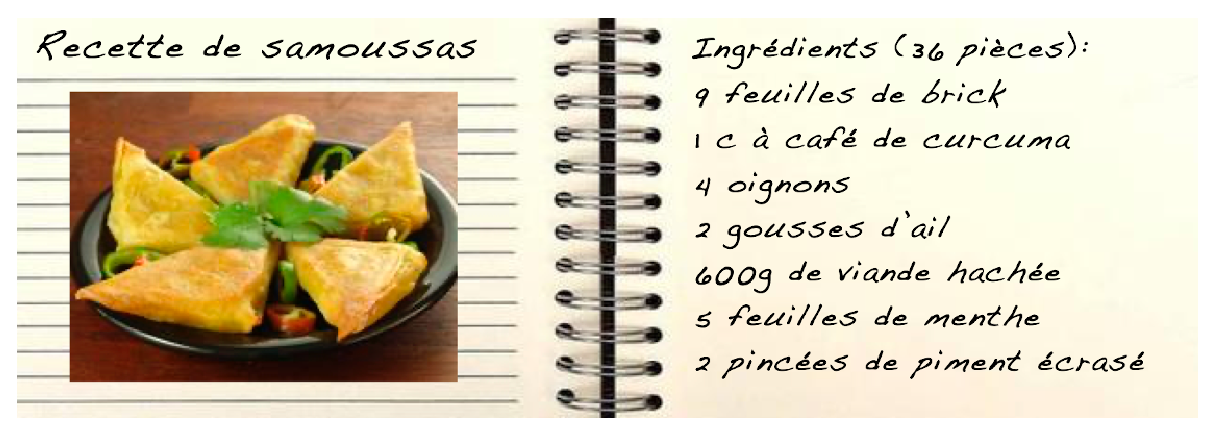
\includegraphics[width=17cm]{samoussas}
   \end{center}
   Le cuisinier a déjà dans sa cuisine les épices, l'ail et la menthe et il a relevé les prix au supermarché du coin : \\
   \begin{center}
      \parbox{7.5cm}{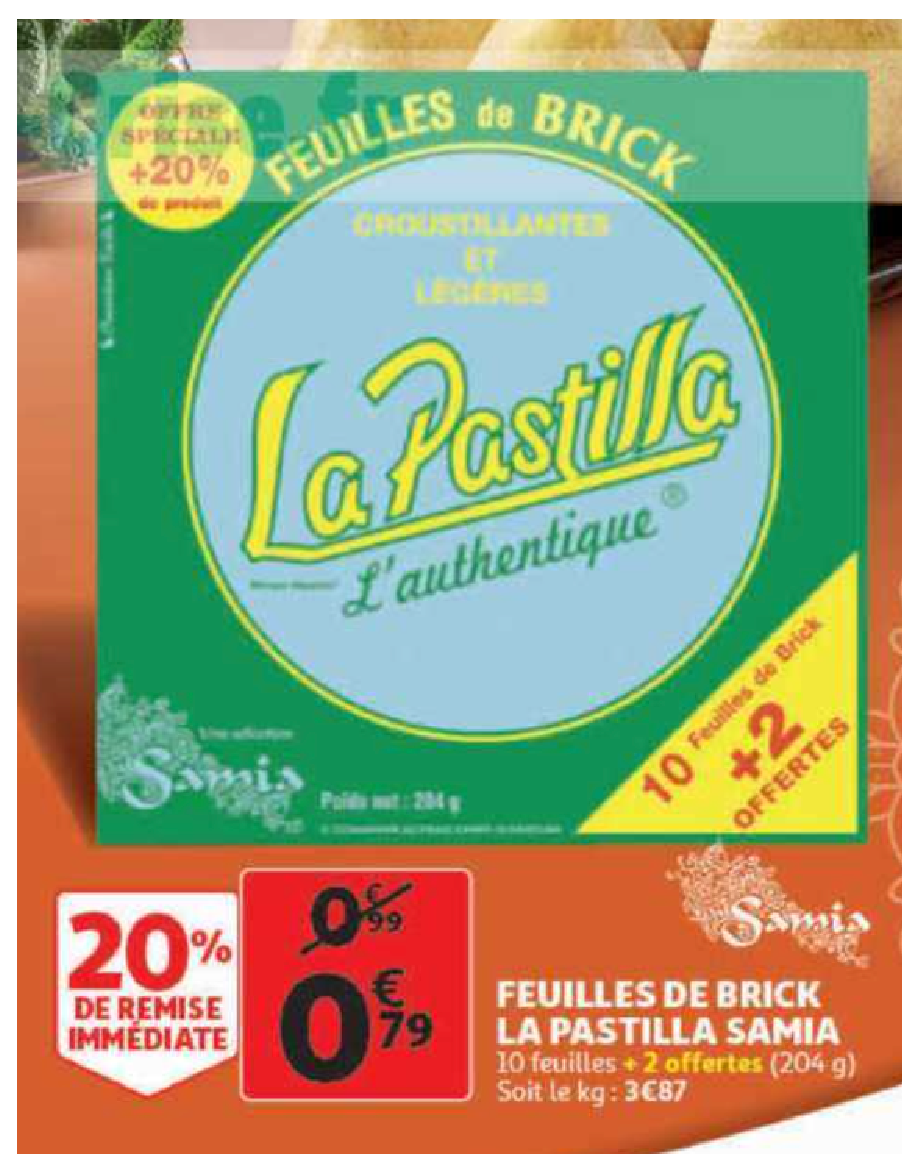
\includegraphics[width=7.5cm]{brick}} \qquad \parbox{8cm}{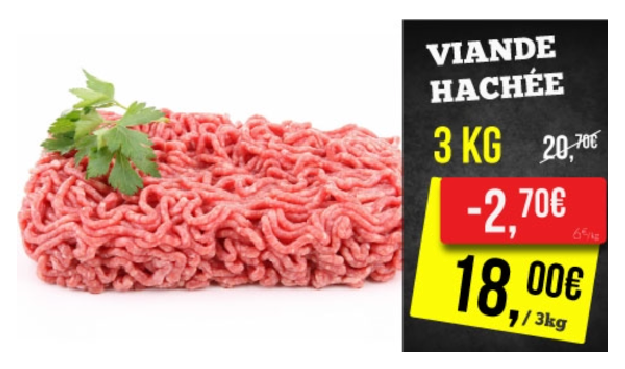
\includegraphics[width=8cm]{viande} \\ [3mm]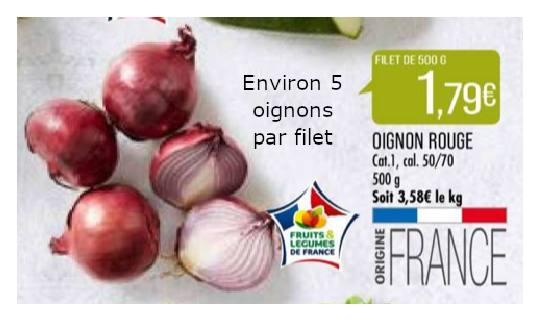
\includegraphics[width=8cm]{oignons}}
   \end{center}
   \medskip
   \begin{cadre}[B2][F4]
      À combien revient la confection des samoussas ? 
   \end{cadre}
   Par groupes de trois ou quatre, proposer une affiche expliquant les achats du cuisinier.
    
   \vfill\hfill{\it\footnotesize Source : inspiré de \href{https://irem.univ-reunion.fr/IMG/pdf/apprendre_avec_taches_complexes_au_cycle_3.pdf}{Apprendre avec ls tâches complexes}}

